\documentclass{article}
\usepackage[utf8]{inputenc}
\usepackage{natbib}
%\bibliographystyle{agsm}
\usepackage{graphicx}

\title{Why Penguins Are Great}
\author{Peter}
\date{June 2019}

\begin{document}
\maketitle

\section{Introduction}

I think that penguins are great and I would like to tell you why.

\subsection{Penguin Details}

Figure \ref{fig:penguin} shows a picture of a penguin. 
\begin{figure}[h!]
	\centering
	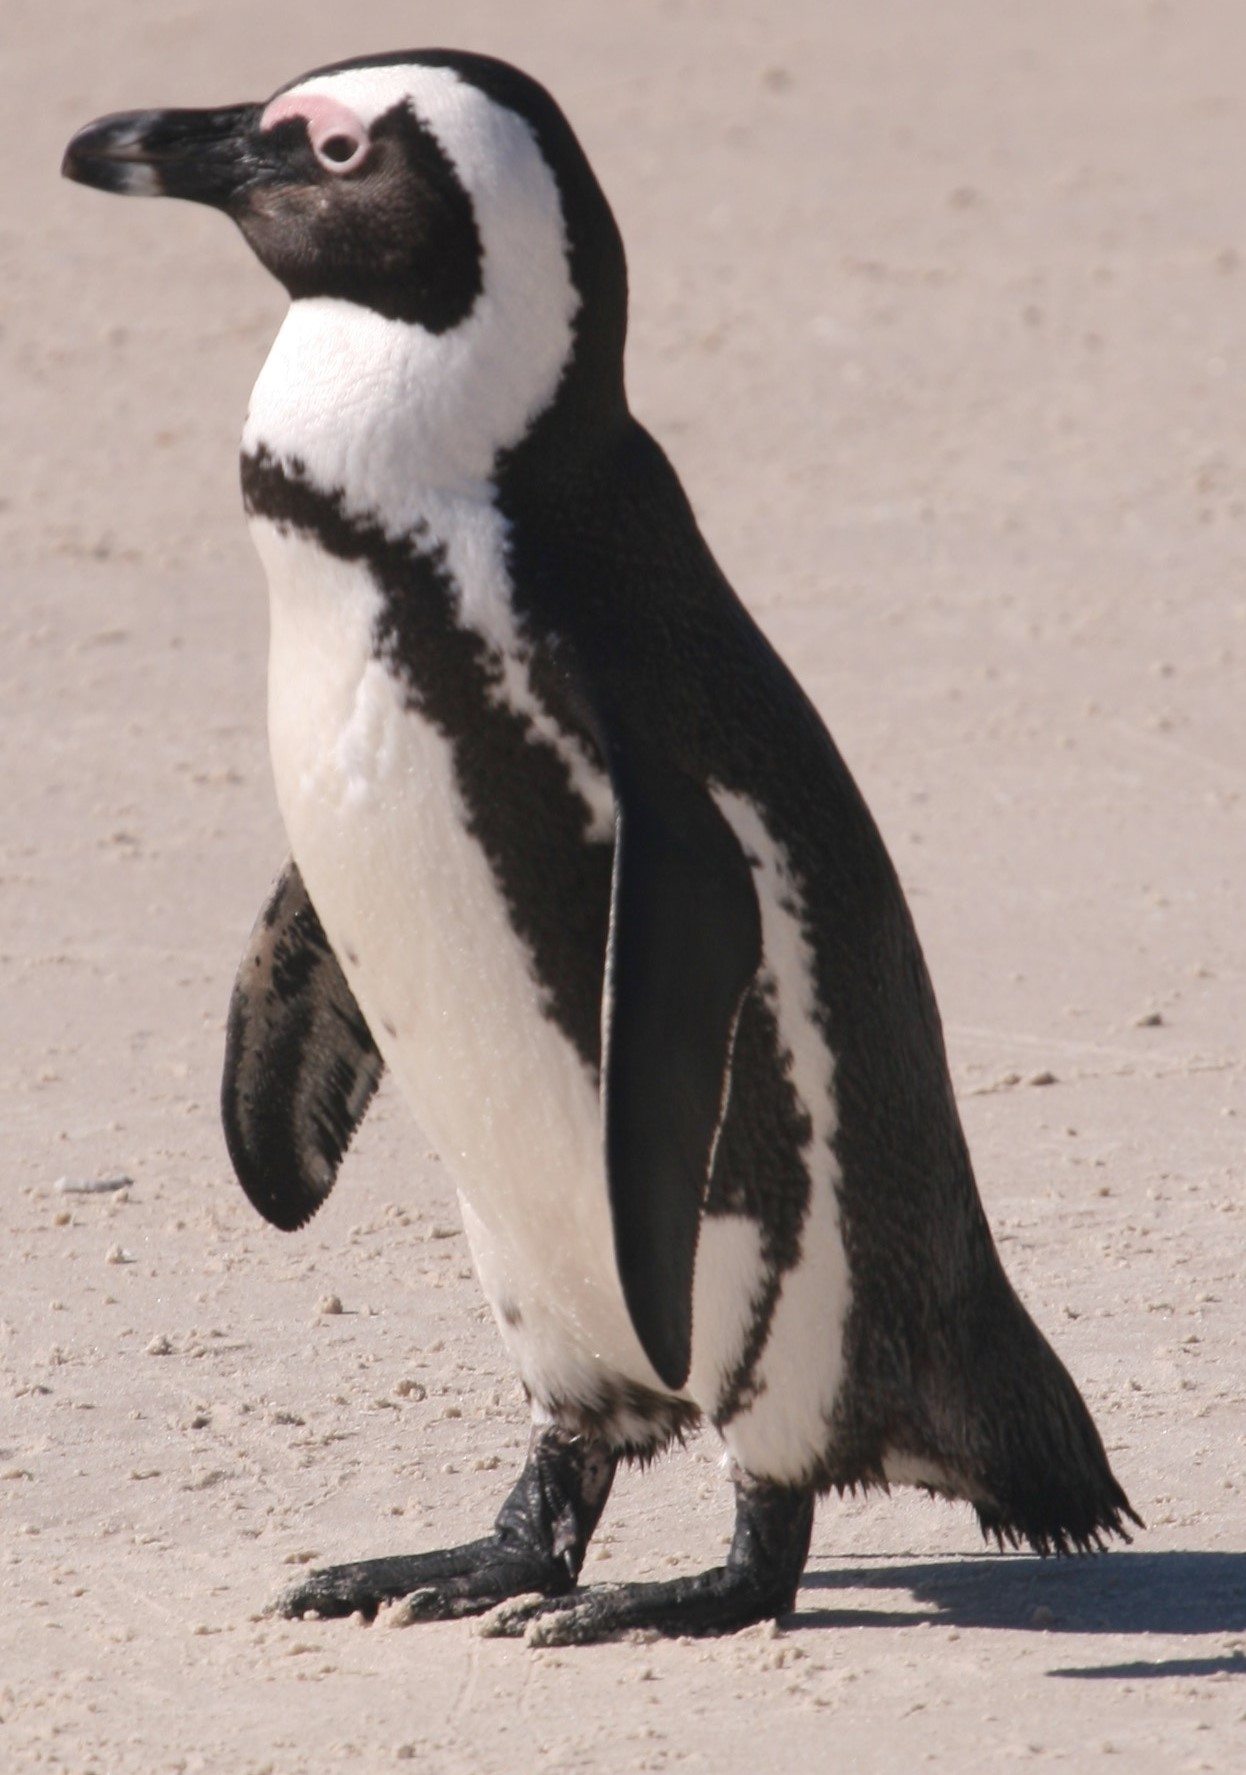
\includegraphics[scale=0.15]{figures/penguin}
	\caption{This is a picture of a penguin. They are fabulous.}
	\label{fig:penguin}
\end{figure}

Other people think that penguins are great too \cite{Mattern2018}.

%Add in a plot of penguin populations here. The data comes from 

\bibliographystyle{plain}
\bibliography{references}

\end{document}